\documentclass{standalone}
\usepackage{tikz}
\usetikzlibrary{patterns, positioning}
\usepackage[sfdefault]{ClearSans} %% option 'sfdefault' activates Clear Sans as the default text font
\usepackage[T1]{fontenc}

\begin{document}
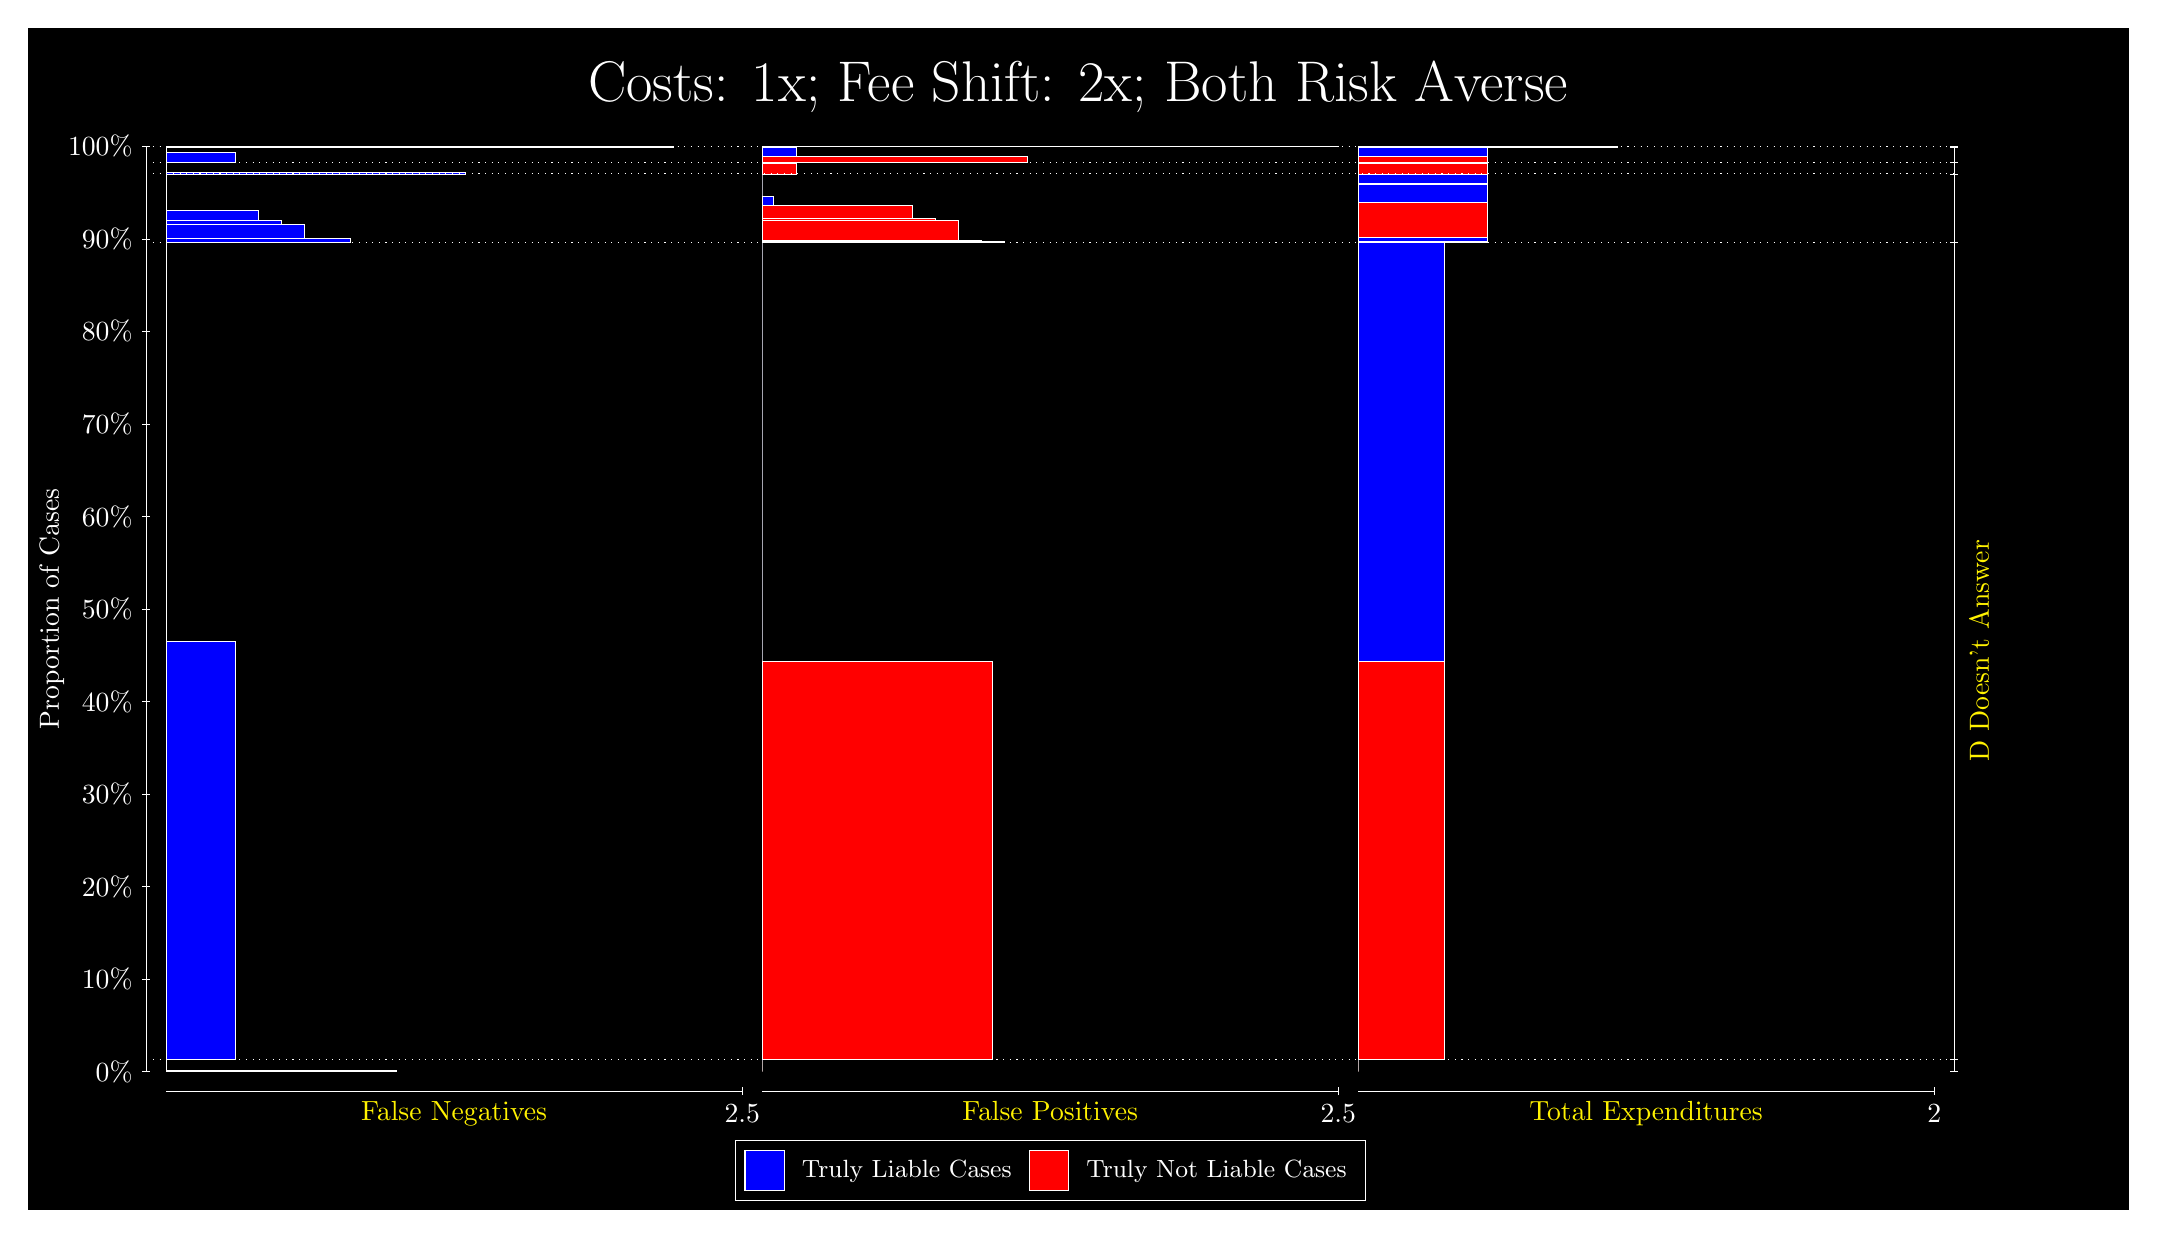
\begin{tikzpicture}
\draw[fill=black] (0,0) rectangle (26.667,15);
\draw[text=white] (0,13.5) rectangle (26.667,15) node[midway] {\huge Costs: 1x; Fee Shift: 2x; Both Risk Averse};
\draw[white, very thin] (1.5,1.75) -- (1.5,13.5);
\node[rotate=90, text=white, anchor=center] at (0.3, 7.625) {Proportion of Cases};
\draw[white, very thin] (1.45,1.75) -- (1.55,1.75);
\node[text=white, anchor=east] at (1.45, 1.75) {0\%};
\draw[white, very thin] (1.45,2.925) -- (1.55,2.925);
\node[text=white, anchor=east] at (1.45, 2.925) {10\%};
\draw[white, very thin] (1.45,4.1) -- (1.55,4.1);
\node[text=white, anchor=east] at (1.45, 4.1) {20\%};
\draw[white, very thin] (1.45,5.275) -- (1.55,5.275);
\node[text=white, anchor=east] at (1.45, 5.275) {30\%};
\draw[white, very thin] (1.45,6.45) -- (1.55,6.45);
\node[text=white, anchor=east] at (1.45, 6.45) {40\%};
\draw[white, very thin] (1.45,7.625) -- (1.55,7.625);
\node[text=white, anchor=east] at (1.45, 7.625) {50\%};
\draw[white, very thin] (1.45,8.8) -- (1.55,8.8);
\node[text=white, anchor=east] at (1.45, 8.8) {60\%};
\draw[white, very thin] (1.45,9.975) -- (1.55,9.975);
\node[text=white, anchor=east] at (1.45, 9.975) {70\%};
\draw[white, very thin] (1.45,11.15) -- (1.55,11.15);
\node[text=white, anchor=east] at (1.45, 11.15) {80\%};
\draw[white, very thin] (1.45,12.325) -- (1.55,12.325);
\node[text=white, anchor=east] at (1.45, 12.325) {90\%};
\draw[white, very thin] (1.45,13.5) -- (1.55,13.5);
\node[text=white, anchor=east] at (1.45, 13.5) {100\%};

\draw[white, very thin] (24.457,1.75) -- (24.457,13.5);
\draw[white, very thin] (24.407,1.75) -- (24.507,1.75);
\node[anchor=west] at (24.407, 1.75) {};
\draw[white, very thin] (24.407,1.8993) -- (24.507,1.8993);
\node[anchor=west] at (24.407, 1.8993) {};
\draw[white, very thin] (24.407,12.281) -- (24.507,12.281);
\node[anchor=west] at (24.407, 12.281) {};
\draw[white, very thin] (24.407,13.15) -- (24.507,13.15);
\node[anchor=west] at (24.407, 13.15) {};
\draw[white, very thin] (24.407,13.3) -- (24.507,13.3);
\node[anchor=west] at (24.407, 13.3) {};
\draw[white, very thin] (24.407,13.494) -- (24.507,13.494);
\node[anchor=west] at (24.407, 13.494) {};
\draw[white, very thin] (24.407,13.498) -- (24.507,13.498);
\node[anchor=west] at (24.407, 13.498) {};
\draw[white, very thin] (24.407,13.5) -- (24.507,13.5);
\node[anchor=west] at (24.407, 13.5) {};

\draw[white, very thin, fill=blue] (1.75,1.75) rectangle (4.6775,1.7657);
\draw[white, very thin, fill=red] (1.75,1.7657) rectangle (1.75,1.8993);
\draw[white, very thin, fill=blue] (1.75,1.8993) rectangle (2.6283,7.2162);
\draw[white, very thin, fill=red] (1.75,7.2162) rectangle (1.75,12.281);
\draw[white, very thin, fill=blue] (1.75,12.281) rectangle (4.092,12.332);
\draw[white, very thin, fill=blue] (1.75,12.332) rectangle (3.7993,12.334);
\draw[white, very thin, fill=blue] (1.75,12.334) rectangle (3.5065,12.51);
\draw[white, very thin, fill=blue] (1.75,12.51) rectangle (3.2138,12.564);
\draw[white, very thin, fill=blue] (1.75,12.564) rectangle (2.921,12.685);
\draw[white, very thin, fill=red] (1.75,12.685) rectangle (1.75,13.15);
\draw[white, very thin, fill=blue] (1.75,13.15) rectangle (5.5558,13.167);
\draw[white, very thin, fill=red] (1.75,13.167) rectangle (1.75,13.3);
\draw[white, very thin, fill=blue] (1.75,13.3) rectangle (2.6283,13.419);
\draw[white, very thin, fill=red] (1.75,13.419) rectangle (1.75,13.494);
\draw[white, very thin, fill=blue] (1.75,13.494) rectangle (8.1906,13.495);
\draw[white, very thin, fill=red] (1.75,13.495) rectangle (1.75,13.498);
\draw[white, very thin, fill=red] (1.75,13.498) rectangle (1.75,13.499);
\draw[white, very thin, fill=blue] (1.75,13.499) rectangle (1.75,13.5);
\draw[white, very thin, fill=red] (9.3189,1.75) rectangle (9.3189,1.8836);
\draw[white, very thin, fill=blue] (9.3189,1.8836) rectangle (9.3189,1.8993);
\draw[white, very thin, fill=red] (9.3189,1.8993) rectangle (12.246,6.9639);
\draw[white, very thin, fill=blue] (9.3189,6.9639) rectangle (9.3189,12.281);
\draw[white, very thin, fill=red] (9.3189,12.281) rectangle (12.393,12.296);
\draw[white, very thin, fill=red] (9.3189,12.296) rectangle (12.1,12.304);
\draw[white, very thin, fill=red] (9.3189,12.304) rectangle (11.807,12.559);
\draw[white, very thin, fill=red] (9.3189,12.559) rectangle (11.515,12.582);
\draw[white, very thin, fill=red] (9.3189,12.582) rectangle (11.222,12.745);
\draw[white, very thin, fill=blue] (9.3189,12.745) rectangle (9.4652,12.867);
\draw[white, very thin, fill=blue] (9.3189,12.867) rectangle (9.3189,13.15);
\draw[white, very thin, fill=red] (9.3189,13.15) rectangle (9.758,13.284);
\draw[white, very thin, fill=blue] (9.3189,13.284) rectangle (9.3189,13.3);
\draw[white, very thin, fill=red] (9.3189,13.3) rectangle (12.686,13.375);
\draw[white, very thin, fill=blue] (9.3189,13.375) rectangle (9.758,13.494);
\draw[white, very thin, fill=red] (9.3189,13.494) rectangle (9.3189,13.497);
\draw[white, very thin, fill=blue] (9.3189,13.497) rectangle (9.3189,13.498);
\draw[white, very thin, fill=red] (9.3189,13.498) rectangle (16.638,13.499);
\draw[white, very thin, fill=blue] (9.3189,13.499) rectangle (13.71,13.5);
\draw[white, very thin, fill=red] (16.888,1.75) rectangle (16.888,1.8836);
\draw[white, very thin, fill=blue] (16.888,1.8836) rectangle (16.888,1.8993);
\draw[white, very thin, fill=red] (16.888,1.8993) rectangle (17.986,6.9639);
\draw[white, very thin, fill=blue] (16.888,6.9639) rectangle (17.986,12.281);
\draw[white, very thin, fill=red] (16.888,12.281) rectangle (18.534,12.289);
\draw[white, very thin, fill=blue] (16.888,12.289) rectangle (18.534,12.344);
\draw[white, very thin, fill=red] (16.888,12.344) rectangle (18.534,12.785);
\draw[white, very thin, fill=blue] (16.888,12.785) rectangle (18.534,13.014);
\draw[white, very thin, fill=red] (16.888,13.014) rectangle (18.534,13.029);
\draw[white, very thin, fill=blue] (16.888,13.029) rectangle (18.534,13.15);
\draw[white, very thin, fill=red] (16.888,13.15) rectangle (18.534,13.284);
\draw[white, very thin, fill=blue] (16.888,13.284) rectangle (18.534,13.3);
\draw[white, very thin, fill=red] (16.888,13.3) rectangle (18.534,13.375);
\draw[white, very thin, fill=blue] (16.888,13.375) rectangle (18.534,13.494);
\draw[white, very thin, fill=red] (16.888,13.494) rectangle (20.181,13.497);
\draw[white, very thin, fill=blue] (16.888,13.497) rectangle (20.181,13.498);
\draw[white, very thin, fill=red] (16.888,13.498) rectangle (20.181,13.499);
\draw[white, very thin, fill=blue] (16.888,13.499) rectangle (20.181,13.5);
\draw[white, dotted] (1.5,1.8993) -- (24.457,1.8993);
\draw[white, dotted] (1.5,12.281) -- (24.457,12.281);
\draw[white, dotted] (1.5,13.15) -- (24.457,13.15);
\draw[white, dotted] (1.5,13.3) -- (24.457,13.3);
\draw[white, dotted] (1.5,13.494) -- (24.457,13.494);
\draw[white, dotted] (1.5,13.498) -- (24.457,13.498);
\draw[white, very thin] (1.75,1.5) -- (9.0689,1.5);
\node[text=yellow, anchor=north] at (5.4094, 1.5) {False Negatives};
\draw[white, very thin] (9.0689,1.45) -- (9.0689,1.55);
\node[text=white, anchor=north] at (9.0689, 1.45) {2.5};

\draw[white, very thin] (9.3189,1.5) -- (16.638,1.5);
\node[text=yellow, anchor=north] at (12.978, 1.5) {False Positives};
\draw[white, very thin] (16.638,1.45) -- (16.638,1.55);
\node[text=white, anchor=north] at (16.638, 1.45) {2.5};

\draw[white, very thin] (16.888,1.5) -- (24.207,1.5);
\node[text=yellow, anchor=north] at (20.547, 1.5) {Total Expenditures};
\draw[white, very thin] (24.207,1.45) -- (24.207,1.55);
\node[text=white, anchor=north] at (24.207, 1.45) {2};


\node[text=yellow, centered, rotate=90] at (24.777, 7.0901) {D Doesn't Answer};






\draw (12.978300999999998,1.5) node[draw=none] (baseCoordinate) {};
\begin{scope}[align=center]
        \matrix[scale=0.5, draw=white, below=0.5cm of baseCoordinate, nodes={draw}, column sep=0.1cm]{
            \node[rectangle, draw, minimum width=0.5cm, minimum height=0.5cm, fill=blue] {}; &
            \node[draw=none, font=\small, text=white] (B) {Truly Liable Cases}; &
            \node[rectangle, draw, minimum width=0.5cm, minimum height=0.5cm, fill=red] {}; &
            \node[draw=none, font=\small, text=white] (B) {Truly Not Liable Cases}; \\
            };
\end{scope}

\end{tikzpicture}
\end{document}